\documentclass[10pt,a4paper]{article}
\usepackage[margin=21mm,headheight=15pt]{geometry}
\usepackage[T1]{fontenc}
\usepackage{lmodern,amsmath,amssymb,tikz,graphicx,hyperref,fancyhdr,enumitem}
\usetikzlibrary{arrows.meta,positioning,calc,decorations.pathmorphing}
\definecolor{ink}{RGB}{20,53,78}
\hypersetup{colorlinks=true,urlcolor=ink,linkcolor=ink}
\setlength{\parindent}{0pt}\setlength{\parskip}{5pt}
\emergencystretch=3em
\pagestyle{fancy}\fancyhf{}\fancyfoot[C]{\thepage}
\renewcommand{\headrulewidth}{.3pt}
\newcommand{\task}[2]{\par\medskip{\color{ink}\Large\bfseries #1. #2}\par\smallskip}
\newcommand{\answer}{\par\smallskip\textbf{Worked reasoning.} }
\setlist[enumerate]{label=\textbf{(\alph*)},leftmargin=7mm,itemsep=7pt}
\begin{document}
\fancyhead[L]{\small Control of Dynamical Systems}
\fancyhead[R]{\small Laboratory 04}
{\color{ink}\LARGE\bfseries Laboratory 04}\par
{\large A passive notch filter and component tolerance}\par
\textbf{Worked solutions -- five integrated problems}\par
{\small\textbf{Evidence boundary.} Original hypothetical scenarios. Derive, calculate and justify decisions; every numerical record is synthetic. Figures are conceptual and not to scale.}
\smallskip\textbf{Shared nominal data.} Nominal series RLC network: $R=10\,\Omega$, $L=0.01$ H, $C=100\,\mu$F. Input is total applied voltage; output spans the combined inductor and capacitor. Components are ideal unless a part adds loss or tolerance.
\task{1}{Selecting the measured voltage in a real circuit}
A series RLC network is driven by an ideal voltage source. The probe spans the inductor and capacitor together, not the capacitor alone. Read the physical measurement terminals before writing the transfer.
\begin{center}\resizebox{\ifdim\width>.98\linewidth.98\linewidth\else\width\fi}{!}{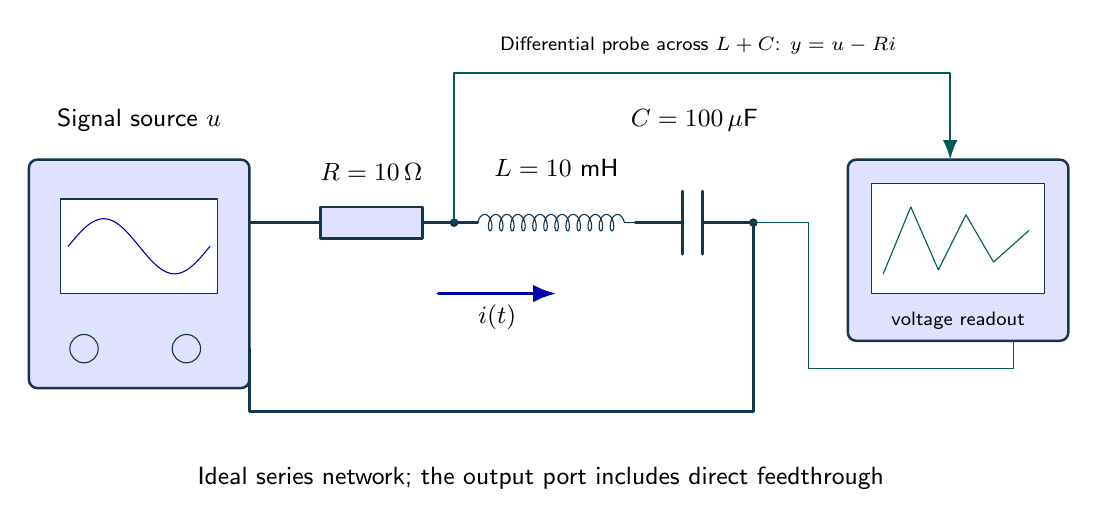
\begin{tikzpicture}[
font=\sffamily\small,>=Latex,line cap=round,line join=round,
wall/.style={draw=ink,line width=1.2pt,fill=blue!5},
water/.style={fill=cyan!25,draw=none},
metal/.style={draw=ink,fill=blue!12,line width=.9pt},
flow/.style={->,draw=blue!65!black,line width=1.2pt},
heat/.style={->,draw=orange!85!black,line width=1.1pt},
measure/.style={->,draw=teal!70!black,line width=.9pt},
dim/.style={<->,draw=ink!65,line width=.6pt},
spring/.style={draw=ink,decorate,decoration={coil,aspect=.5,segment length=4pt,amplitude=3pt}},
wire/.style={draw=ink,line width=1pt},
lab/.style={align=center,font=\sffamily\small},
smalllab/.style={align=center,font=\sffamily\scriptsize}]

\draw[metal,rounded corners=3pt](.3,1.1)rectangle(3.1,4);
\draw[fill=white,draw=ink](.7,2.3)rectangle(2.7,3.5);
\draw[blue!70!black,domain=.8:2.6,samples=60]plot(\x,{2.9+.35*sin(360*(\x-.8)/1.8)});
\draw[ink](1,1.6)circle(.18)(2.3,1.6)circle(.18);
\node[lab]at(1.7,4.5){Signal source $u$};
\draw[wire](3.1,3.2)--(4,3.2);
\draw[metal](4,3)rectangle(5.3,3.4);
\node[lab]at(4.65,3.85){$R=10\,\Omega$};
\draw[wire](5.3,3.2)--(6,3.2);
\draw[spring](6,3.2)--(8,3.2);
\draw[wire](8,3.2)--(8.6,3.2);
\draw[wire](8.6,2.8)--(8.6,3.6)(8.85,2.8)--(8.85,3.6);
\draw[wire](8.85,3.2)--(9.5,3.2)--(9.5,.8)--(3.1,.8)--(3.1,1.6);
\node[lab]at(7,3.9){$L=10$ mH};
\node[lab]at(8.75,4.5){$C=100\,\mu$F};
\draw[flow](5.5,2.3)--(7,2.3)node[midway,below]{$i(t)$};
\draw[metal,rounded corners=3pt](10.7,1.7)rectangle(13.5,4);
\draw[fill=white,draw=ink](11,2.3)rectangle(13.2,3.7);
\draw[teal!70!black](11.15,2.55)--(11.5,3.4)--(11.85,2.6)--(12.2,3.3)--(12.55,2.7)--(13,3.1);
\node[smalllab]at(12.1,1.95){voltage readout};
\fill[ink](5.7,3.2)circle(.055)(9.5,3.2)circle(.055);
\draw[measure](5.7,3.2)--(5.7,5.1)--(12,5.1)--(12,4);
\draw[teal!70!black](9.5,3.2)--(10.2,3.2)--(10.2,1.35)--(12.8,1.35)--(12.8,1.7);
\node[smalllab]at(8.8,5.45){Differential probe across $L+C$: $y=u-Ri$};
\node[lab]at(6.8,-.05){Ideal series network; the output port includes direct feedthrough};
\end{tikzpicture}
}\par{\small A source excites the series RLC network; an ideal differential probe spans the combined inductor and capacitor. Measuring only the capacitor would produce a different transfer function. Wire placement is schematic.}\end{center}
\begin{enumerate}
\item A voltage source drives series $R=10\,\Omega$, $L=0.01$ H and $C=100\,\mu$F. Output is the sum of inductor and capacitor voltages. Derive $H(s)$ and its DC and high-frequency gains.
\answer The series impedance is $R+sL+1/(sC)$ and the output impedance is $sL+1/(sC)$. Their ratio gives $H=(LCs^2+1)/(LCs^2+RCs+1)$. Both DC and high-frequency gains are one. The latter follows from equal leading coefficients, not from a low-pass approximation. This is an ideal unloaded voltage measurement across the combined reactive elements.
\item Find the notch frequency, damping ratio, poles and zeros for the nominal circuit. State whether a zero on the imaginary axis makes the circuit internally unstable.
\answer Here $LC=10^{-6}$ and $RC=10^{-3}$, so $\omega_0=1/\sqrt{LC}=1000$ rad/s and $\zeta=(R/2)\sqrt{C/L}=0.5$. The poles solve $s^2+1000s+10^6=0$, giving $-500\pm j500\sqrt3$. The zeros are $\pm j1000$. Stability is determined by the poles: these have negative real parts. Imaginary-axis transmission zeros represent cancellation at one output frequency, not unstable internal dynamics.
\item Derive the capacitor-voltage transfer for the same components and compare its numerator and direct feedthrough with those of the specified combined output. Explain why the poles remain unchanged.
\answer For capacitor voltage, $H_C=1/(LCs^2+RCs+1)$, so its DC gain is one and its high-frequency gain is zero. The combined output has $H=(LCs^2+1)/(LCs^2+RCs+1)$ and high-frequency gain one. The same state dynamics and denominator are used, but the output equation changes. An output zero is not evidence that a physical energy-storage element or internal mode has disappeared.
\end{enumerate}

\newpage
\task{2}{A zero output with nonzero circulating energy}
Compare sinusoidal resonance with the response to a sudden voltage step. Both tests use the same passive network, but expose different aspects of the measured output.
\begin{enumerate}
\item At the notch frequency, the source has sinusoidal peak voltage 2 V. Find peak current, peak inductor and capacitor voltages, and the maximum energy in each reactive component.
\answer At resonance the reactive impedances cancel, so $I_{pk}=2/10=0.2$ A. Each reactive voltage has peak magnitude $\omega_0 L I_{pk}=2$ V; their phasors oppose. Maximum inductor energy is $LI_{pk}^2/2=0.0002$ J. The capacitor energy maximum is $CV_{C,pk}^2/2=0.0002$ J. The output voltage sum is zero, but current and stored energies are nonzero; the two energy maxima occur at different phases.
\item Derive the nominal unit-step output. Find its initial and final values, and explain why neither contradicts rejection of a sinusoid at 1000 rad/s.
\answer Write $H=1-1000s/(s^2+1000s+10^6)$. For a unit step, $Y=1/s-1000/(s^2+1000s+10^6)$. Therefore $y=1-(2/\sqrt3)e^{-500t}\sin(500\sqrt3\,t)$ for $t\ge0$. Both $y(0^+)$ and $y(\infty)$ equal one. A step includes a DC component, which passes with unit gain. The notch removes one steady sinusoidal frequency, not all inputs or all transient motion.
\item At sinusoidal resonance with a 2 V source peak, write magnetic and electric energy as functions of phase. Determine their sum and explain whether both energy maxima occur simultaneously.
\answer The resonant current peak is 0.2 A and capacitor-voltage peak is 2 V. With current phase $\varphi$, $E_L=\tfrac12L(0.2)^2\cos^2\varphi=0.0002\cos^2\varphi$ J and $E_C=\tfrac12C(2)^2\sin^2\varphi=0.0002\sin^2\varphi$ J. The sum is 0.0002 J, although each energy alternates between zero and that maximum. Their maxima occur a quarter cycle apart. A canceled output voltage therefore coexists with energy exchange and resistor dissipation.
\end{enumerate}

\newpage
\task{3}{When component tolerance and winding loss spoil the notch}
The ideal cancellation is challenged by a capacitor tolerance and a lossy inductor. Separate frequency detuning from an output floor caused by resistance.
\begin{center}\resizebox{\ifdim\width>.98\linewidth.98\linewidth\else\width\fi}{!}{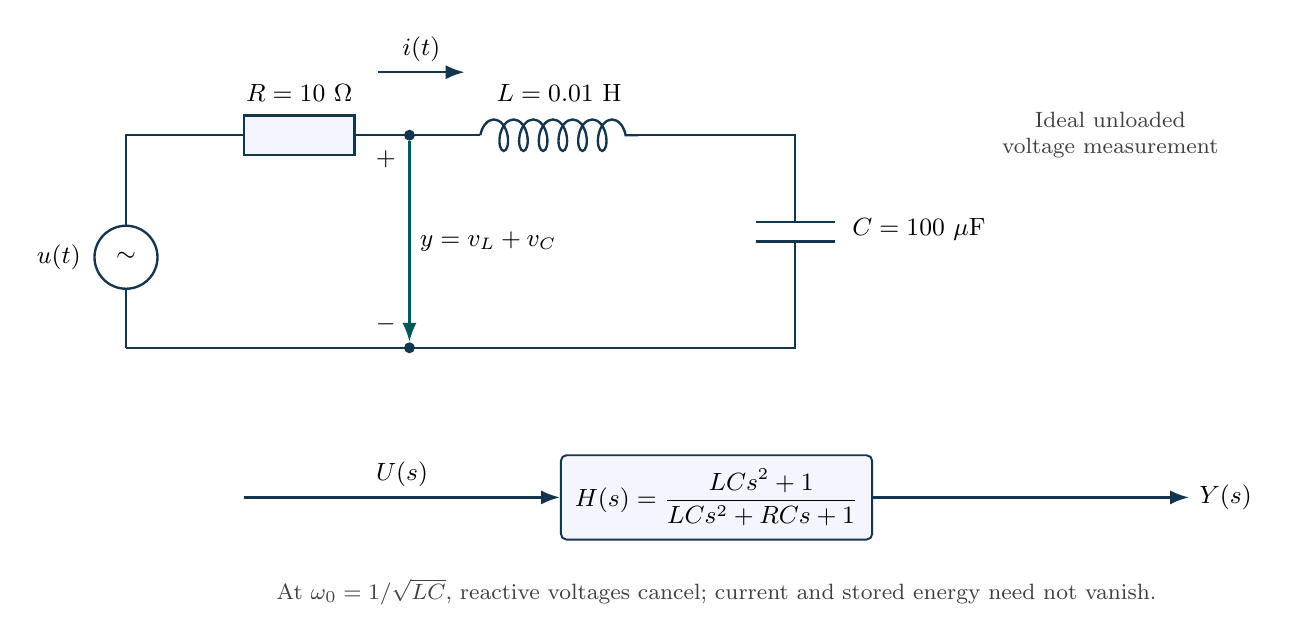
\begin{tikzpicture}[x=1cm,y=1cm,>=Latex,font=\small,
block/.style={draw=ink,fill=blue!4,rounded corners=2pt,minimum height=9mm,align=center,line width=.7pt,inner sep=5pt},
sum/.style={circle,draw=ink,fill=white,minimum size=6mm,inner sep=0pt,line width=.7pt},
sig/.style={->,draw=ink,line width=.85pt},
fb/.style={->,draw=teal!70!black,line width=.85pt},
dist/.style={->,draw=orange!75!black,line width=.85pt},
tap/.style={circle,fill=ink,inner sep=1.4pt},
note/.style={font=\footnotesize,align=center,text=black!75}]

\draw[draw=ink,line width=.85pt](.5,.3)--(.5,1.05);
\draw[draw=ink,line width=.85pt](.5,1.45)circle(.4);
\node at(.5,1.45){$\sim$};
\draw[draw=ink,line width=.85pt](.5,1.85)--(.5,3)--(2,3);
\node[left]at(.05,1.45){$u(t)$};
\draw[draw=ink,fill=blue!4,line width=.85pt](2,2.75)rectangle(3.4,3.25);
\node[above]at(2.7,3.3){$R=10\ \Omega$};
\draw[draw=ink,line width=.85pt](3.4,3)--(5,3);
\draw[decorate,decoration={coil,aspect=.55,segment length=2.5mm,amplitude=2mm},line width=.85pt,draw=ink](5,3)--(7,3);
\node[above]at(6,3.3){$L=0.01\ \mathrm{H}$};
\draw[draw=ink,line width=.85pt](7,3)--(9,3)--(9,1.9);
\draw[line width=.85pt,draw=ink](8.5,1.9)--(9.5,1.9)(8.5,1.65)--(9.5,1.65);
\draw[line width=.85pt,draw=ink](9,1.65)--(9,.3)--(.5,.3);
\node[right]at(9.6,1.8){$C=100\ \mu\mathrm{F}$};
\draw[sig](3.7,3.8)--node[above]{$i(t)$}(4.8,3.8);
\node[tap](a)at(4.1,3){};\node[tap](b)at(4.1,.3){};
\draw[fb](a)--node[right]{$y=v_L+v_C$}(b);
\node at(3.8,2.7){$+$};\node at(3.8,.6){$-$};
\node[note]at(13,3){Ideal unloaded\\voltage measurement};
\node[block](h)at(8,-1.6){$H(s)=\dfrac{LCs^2+1}{LCs^2+RCs+1}$};
\draw[sig](2,-1.6)--node[above]{$U(s)$}(h);
\draw[sig](h)--(14,-1.6)node[right]{$Y(s)$};
\node[note]at(8,-2.8){At $\omega_0=1/\sqrt{LC}$, reactive voltages cancel; current and stored energy need not vanish.};

\end{tikzpicture}
}\par{\small Series RLC network with output measured across L and C together. The output probe spans those two components, not the whole source.}\end{center}
\begin{enumerate}
\item With L and R fixed, let capacitance be 10 percent low or high. Calculate both notch frequencies. If the input remains at 1000 rad/s, give a formula for the residual output magnitude for a capacitance factor $f=C/C_0$.
\answer The notch shifts to $1000/\sqrt f$ rad/s: approximately 1054.09 for $f=0.9$ and 953.46 for $f=1.1$. At the old notch, $LC\omega^2=f$ and $RC\omega=f$, hence $|H(j1000)|=|1-f|/\sqrt{(1-f)^2+f^2}$. The corresponding magnitudes are about 0.11043 and 0.09054. A shifted notch does not cancel the original fixed-frequency interference exactly.
\item Add winding resistance $r_L=1\,\Omega$ in series with the ideal inductor. The output spans that winding resistance, inductor and capacitor. Derive the new transfer and evaluate the output at the nominal resonant frequency.
\answer The measured impedance is $r_L+sL+1/(sC)$, so $H_{loss}=(LCs^2+r_LCs+1)/(LCs^2+(R+r_L)Cs+1)$. At $\omega_0$, ideal reactances cancel, leaving magnitude $r_L/(R+r_L)=1/11\approx0.09091$, about $-20.83$ dB. This evaluates the response at the nominal resonance; it need not be the exact frequency of minimum magnitude. The nonzero winding voltage limits cancellation at that frequency.
\item At the nominal resonance, require output magnitude strictly below 0.05 when only winding resistance varies and $R=10\,\Omega$. Derive the permitted resistance interval and assess a 1 $\Omega$ winding.
\answer At the ideal reactive cancellation frequency, the output across the winding plus LC section has magnitude $r_L/(R+r_L)$. For nonnegative $r_L$, the requirement is $r_L/(10+r_L)<0.05$, or $0\le r_L<10/19\simeq0.52632\,\Omega$. A 1 $\Omega$ winding produces $1/11\simeq0.09091$ and fails. Simultaneous capacitance error must be evaluated through the complex impedance; its magnitude cannot in general be added directly to this loss floor.
\end{enumerate}

\newpage
\task{4}{Changing damping without moving the nominal notch}
The resistor can be changed without changing ideal L or C. Relate pole damping to the useful frequency interval of attenuation.
\begin{enumerate}
\item Choose R for critical damping without changing nominal L and C. Determine the resulting poles, and explain what happens to the ideal notch zeros.
\answer Critical damping means $\zeta=1$, so $R=2\sqrt{L/C}=20\,\Omega$. The denominator becomes $(s+1000)^2$ after normalization, giving a repeated pole at $-1000$ s$^{-1}$. The numerator remains $LCs^2+1$, so zeros stay at $\pm j1000$. Resistance changes pole damping and the notch width; in the ideal circuit it does not set the cancellation frequency.
\item Derive the two positive frequencies where the nominal magnitude is $1/\sqrt2$. Show that their product is $\omega_0^2$ and their separation is $R/L$.
\answer Squaring the magnitude condition gives $(1-r^2)^2=(2\zeta r)^2$. The two positive roots are $r_- =\sqrt{1+\zeta^2}-\zeta$ and $r_+=\sqrt{1+\zeta^2}+\zeta$. For $\zeta=0.5$, they are $(\sqrt5-1)/2$ and $(\sqrt5+1)/2$, giving about 618.034 and 1618.034 rad/s. Their product is one and difference is $2\zeta$; therefore $\omega_-\omega_+=\omega_0^2$ and $\omega_+-\omega_-=2\zeta\omega_0=R/L=1000$ rad/s.
\item Require a notch at 1000 rad/s, a half-power notch bandwidth of 800 rad/s and critically damped poles. Keep the nominal L and C and vary only R. Determine the resistance demanded by each requirement and decide whether all three can hold simultaneously.
\answer The fixed reactive elements already give $\omega_0=1/\sqrt{LC}=1000$ rad/s, independently of R. The bandwidth condition gives $R=L(800)=8\,\Omega$, hence $\zeta=(R/2)\sqrt{C/L}=0.4$ and poles $-400\pm j\sqrt{840000}$ s$^{-1}$. Critical damping instead requires $R=2\sqrt{L/C}=20\,\Omega$, giving bandwidth $R/L=2000$ rad/s. No single resistor satisfies both bandwidth and damping requirements. The design must relax one requirement or change the circuit; choosing a compromise value alone does not meet the stated specifications.
\end{enumerate}

\newpage
\task{5}{A state model that preserves the circuit power balance}
Use the circuit states to connect frequency calculations to conservation of energy. Pay attention to the direct contribution of the applied voltage to the selected output.
\begin{enumerate}
\item For the nominal circuit, calculate output magnitude at 500 and 2000 rad/s. Explain the equality using the normalized frequency $r=\omega/\omega_0$.
\answer The magnitude is $|1-r^2|/\sqrt{(1-r^2)^2+(2\zeta r)^2}$. With $\zeta=0.5$, $r=0.5$ gives $0.75/\sqrt{0.8125}=3/\sqrt{13}$. For $r=2$, it gives $3/\sqrt{13}$ again, approximately 0.83205, or $20\log_{10}(3/\sqrt{13})\approx-1.597$ dB. Dividing numerator and denominator by $r^2$ reveals the symmetry under $r\mapsto1/r$.
\item Use capacitor voltage $v_C$ and current $i$ as states and input voltage $u$. Derive A, B, C and D for output equal to the ideal LC voltage sum. Explain the direct feedthrough term.
\answer The equations are $\dot v_C=i/C$ and $\dot i=(u-Ri-v_C)/L$. Thus $A=\begin{bmatrix}0&1/C\\-1/L&-R/L\end{bmatrix}$, $B=[0,1/L]^T$. Since $y=u-Ri$, the output matrices are $C_y=[0,-R]$ and $D=1$. At an ideal voltage step, current is continuous, so the output immediately inherits the input jump. This direct feedthrough agrees with the transfer's unit high-frequency gain.
\item With states $[i,v_C]^T$, derive $\dot E$ for $E=Li^2/2+Cv_C^2/2$. Use it to distinguish passivity from the incorrect assertion that all output magnitudes must be below one.
\answer From $L\dot i=u-Ri-v_C$ and $C\dot v_C=i$, $\dot E=Li\dot i+Cv_C\dot v_C=ui-Ri^2$. The circuit stores supplied energy and dissipates $Ri^2$, establishing the power balance. Passivity concerns supplied power, not a universal bound on every internal voltage ratio: reactive voltages can be amplified near resonance. For the combined output, $y=u-Ri$, the state output equation must retain direct term $D=1$.
\end{enumerate}

\end{document}
